\chapter{Reference}
\label{reference}
This chapter will take an in-depth look at most of the bells and whistles of \texnicle.

\section{Preferences}
\label{reference.prefs}
Access the preference pane just like in any other Mac application: \menu{TeXnicle > Preferences\ldots} (or, if you prefer keyboard shortcuts, \keys{\cmdkey +,} will open the window). There are seven preference categories: General, Typesetting, Fonts \& Colors, Templates, Commands, Palette \& Library, and File Types.

\subsection{General}
\label{reference.prefs.gen}
Several important features are included under the General pane. You can set the number of characters per line, at which point the line will wrap. Alternatively, you can turn wrapping off. When pressing the Tab key, a tab is inserted into the document; this behaviour can be changed from the General tab to insert any number of spaces instead.

\texnicle can insert closing braces automatically when an opening brace is typed, if you so choose. You can also opt to skip closing braces, which means that when the cursor is set immediately before a closing brace and then the \} key is pressed, the editor will simply skip that brace rather than inserting a new one. You may also choose for \texnicle to automatically replace opening quotation marks (\keys{\shiftkey + '}) with two inverted apostrophes (\keys{`}). Line numbering and code folding (for |\begin| and |\end| environments) can be turned on and off here. Line highlighting and the highlighting of matching words can also be edited.

\texnicle is happy to save a project automatically when compiling the document, but if you want to turn off this feature, it is located under the General tab. You can also toggle whether \texnicle restores project tabs when opening a project. Finally, the default file encoding can be set to any one of a number of encoding options. The default is Unicode (UTF-8).

\subsection{Typesetting}
\label{reference.prefs.type}
The second tab in the Preferences window is the Typesetting pane. This concerns the nuts and bolts of \texnicle with features like typesetting (obviously), syntax checking, engines, and the discard of auxiliary files.

Typesetting options include the ability to clear the consoles upon typesetting a document, the number of seconds between Live Updates, and a few other tweaks for the typesetting process. Aside from clearing the console and the amount of time between Live Updates, changes made under the Typesetting subcategory of this preference pane affect the default values of new projects rather than the existing project. This means that changing the default typesetting engine, for example, under this preference pane will not affect the engine used for any existing projects; that option is changed in the Project Settings tab of the Navigator on a by-project basis.

There are many options for syntax checking are possible. These are done with the |chtex| binary from your \LaTeX\ installation. The path for this may need to be re-configured if you do not have a stock installation of MacTeX on your machine. Syntax checking can be turned on and off from this tab under the Typesetting preference pane.

Typesetting engines are edited and created under the Engines tab of the Typesetting pane. Everything that has to do with engines is discussed in section \ref{reference.engines}.

The Trash tab in the Typesetting pane allows you to define which file types (aux, log, bbl, out, dvi, ilg, ps, and so on) are deleted when using the Trash Aux Files feature.

\subsection{Fonts \& Colors}
\label{reference.prefs.fontcol}
This section allows you to change the colours used to highlight \LaTeX\ syntax, the colours used in the editor window, and the fonts used in the editor window and the console. Three levels of differentiation in comments (using the \% symbol) and three levels of markup text (that should be edited later, marked with {\textless} and {\textgreater}) are possible.

\noted{There is an option to colour multi-line arguments under this tab. While this function may be desirable, please note that it is very taxing for \texnicle and may slow down your system.}

\subsection{Templates}
\label{reference.prefs.templates}
The Templates preference pane allows you to create, edit, and delete two kinds of templates: file templates and project templates. File templates are templates that can be used to start new \LaTeX\ documents. \texnicle comes with many default templates installed, but you may also edit these as well as define your own. Project templates create new projects based on a template. \texnicle comes with one project template preinstalled: the article template. After naming your template, this opens a new project window with a file based on the Article file template and creates two folders: \folder Include for files you will include in your document through the main file, and \folder Images for image files you will insert into the document. These can be edited at will. You may also define new project templates or create new templates from existing projects.

\subsection{Commands}
\label{reference.prefs.commands}
The Commands pane is home to many of the powerful and most convenient features \texnicle has to offer. The categories within this pane will be discussed in detail.

The first tab is the Commands tab, which controls command completion. When you begin typing a command, \texnicle can be set to bring up a list of default commands that match what you have typed. This function can be turned on or off from within this pane. When the function is turned off, it will not automatically show the completion list; however, the completion list may still be viewed by clicking \menu{Edit > Smart Complete} or by pressing \keys{\esckey}. The Commands tab is also where you can define custom commands that will appear in this menu.

The second tab controls citation completion. When any citation command (either a default command like |\cite|, |\citet|, etc.\ or a custom command like |\cites|) is typed, \texnicle will show a list of possible citations that match the key you have typed between the braces based on the bibliography files referenced in your document. As with command completion, this function can be turned on and off at will.

The third tab, References, does the same thing for |\label| and |\ref| commands. When typing |\ref| (or a similar referencing command defined by the user and added to this list), a list of labels within the document or project matching what you have typed will be displayed. This can be turned off.

The File tab does the same thing for |\input| and |\include| commands, which can be turned off. The |.tex| file extension is left off, as expected.

Finally, the Begin tab controls an autocomplete list for |\begin{environment}| commands. Default environments are included, but you may add to or delete from this list as you wish. You can also ask \texnicle to auto-insert an |\end{environment}| command when you input a carriage return after beginning an environment.

\subsection{Palette \& Library}
\label{reference.prefs.palettelibrary}
This section controls the paths to scripts use for creating preview images for the palette and library code clippings. Default paths are set up based on a standard MacTeX installation, but these may need to be rewritten if your system has a different installation.

\subsection{File Types}
\label{reference.prefs.filetypes}
This preference pane includes a list of files that \texnicle will recognize as {\TeX} files. You can toggle which documents have syntax highlighting enabled and which files are spell-checked (for more on spell-checking, see section \ref{reference.spellcheck}). By default, the following file types are included: tex, bib, sty, cls, bst.

\section{Engines}
\label{reference.engines}
\texnicle has configurable engines. If you don't need any specialized compiling capabilities, you can simply use the engines supplied by \texnicle by default. If you need more individualized engines, however, you can create your own. \texnicle engines are simple scripts which reside in \directory{/Library/Application Support/TeXnicle/engines}.

A number of variables are passed to these script files from \texnicle. If you create a new engine, the template is preconfigured with the necessary variable set. To start making a new template, click \menu{New} under \menu{Preferences\ldots > Typesetting > Engines}.

\noted{You can only edit engines that you have created yourself. Every time \texnicle opens, it rewrites the default engine files to their former, unchanged version.}

To customize a built-in engine, use the \menu{Duplicate} button under \menu{Preferences\ldots > Typesetting > Engines}. You can then edit the engine script and save it as a new engine.

Under \menu{Preferences\ldots > Typesetting}, you can set the default engine that is used for new projects and documents. You can also specify default values to some of the configuration variables that are passed on to the engines. Not all engines support all configuration variables.

\section{Spell Check}
\label{reference.spellcheck}
Spell-checking is a key feature of \texnicle. Using \href{http://cocoaspell.leuki.com}{http://cocoaspell.leuski.net/}, a Mac OS X implementation of \href{http://aspell.net/}{Aspell}, \texnicle can check the spelling of {\TeX} documents while ignoring \LaTeX\ commands and their arguments. We suggest that you download and install cocoAspell from the developer, turn on {\TeX/\LaTeX} awareness for your chosen dictionaries, and tell \texnicle to use your chosen cocoAspell dictionary when checking your project. This setting is found under the Project Settings tab in the Navigator pane. Spelling checks are conducted every five seconds (in documents that have undergone changes since the last check), and the results are populated under the Spelling tab of the Index part of the Navigator pane.

Only files marked to check spelling under \menu{Preferences\ldots > File Types} will be checked.

\section[Creating Project Templates]{Creating a New \texnicle Project Template}
\label{reference.newtemplate}
After you've laboured for weeks or months setting up your project so that it has everything you need to work from entirely within \texnicle, you may decide to save a version of your project as a project template so you can base other projects on it in the future without reinventing the wheel. This is done by clicking \menu{Project > New Project Template\ldots} from within the project you want to use as a basis for your template. The window in Figure \ref{fig:texnicle-newtemplate} will appear.
\begin{figure}[htbp]
\caption{Creating a Project Template}
\label{fig:texnicle-newtemplate}
\centering
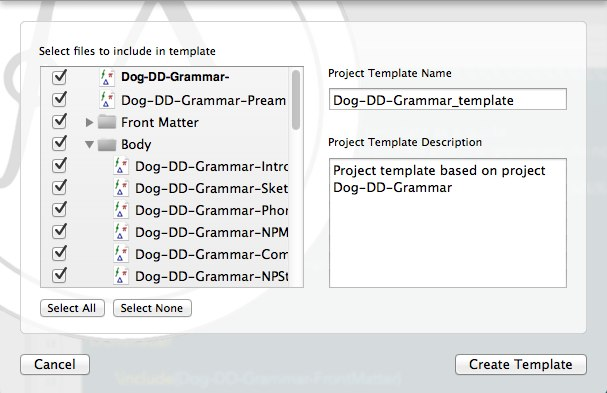
\includegraphics[width=10cm]{TeXnicle-Images/texnicle-newtemplate.jpg}
\end{figure}

From this window you can name the template, provide a description, and select which files in the existing project are ported to the new template.

\section{Project Management}
\label{reference.projectmanagement}
To create a new folder in your project, click the folder icon in the bottom left corner of the Navigators pane or click \menu{Project > New Folder}. You will be given the option to create a Group Folder, which will appear in grey and exist only within the TeXnicle project space, or a Folder on Disk, which will appear in blue and exist on your hard drive. Similarly, you can add a new \TeX\ document by clicking the document icon at the bottom of the Navigators pane or by clicking \menu{Project > New \LaTeX\ File}. The Template Selection window will appear.

\noted{\menu{Project > New File} will create a new file, but you must specify its extension. This function will not create a \TeX\ file unless you add the extension manually.}

\keys{\shiftkey + \cmdkey + A} will allow you to search your computer for an existing file to add to your project. You will be given the option to copy the file to the project folder or simply to reference it from afar. Similarly, \keys{\optkey + \shiftkey + \cmdkey + A} will allow you to add an existing folder. These functions are also available in the \menu{Project} menu or by clicking the gear in the bottom right corner of the Navigators pane.

Changing the main document of your project can be done through the \menu{Project} menu or by \cmdkey-clicking the document in the Project Tree that you want to set. \cmdkey-clicking a file in the Project Tree view will also allow you to rename, remove, or reveal the file.

\section[Clippings Library]{The Clippings Library}
\label{reference.clippings}
The clippings library is one of \texnicle's most economical features. Becoming familiar with clippings and customizing your library is a great way to save time and effort while preparing your document. Recall the Clippings Library window in the Navigators pane:
\begin{figure}[ht]
\centering
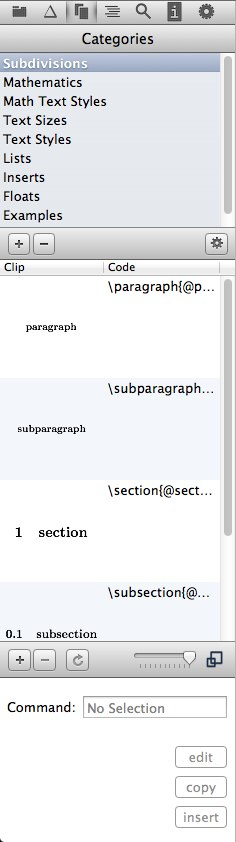
\includegraphics[width=3cm]{TeXnicle-Images/texnicle-clippingslibrary.jpg}
\caption{The Clippings Library pane}
\label{fig:texnicle-clippingslibrary2}
\end{figure}

To add a category of clippings, click the \menu{+} button under ``Categories.'' (For example, the category ``Examples'' in Figure \ref{fig:texnicle-clippingslibrary2} was a custom addition.) To add a clipping to an existing category, click the \menu{+} button under the list of clippings. To edit a clipping, double-click the code.

Adding clippings is as easy as writing the code and then pasting it into a new clipping. After clicking the \menu{+} button, two options are given: ``New clip'' and ``New from pasteboard.'' The former will open a new clipping in the list; double-click to edit. The latter will automatically create a clipping based on copied text.

Once your clip has been created, it's a good idea to set a command for the clip for easy access. This is done in the third panel of the clipping library. To use a clipping by invoking the command, type |#(command-shortcut)| into the editor window. For example, to insert a table into your document quickly and easily, type |#tbl| in the editor window where you want a new table to appear. If the shortcut command is valid, it will be highlighted in yellow as in Figure \ref{fig:texnicle-validclip}.

\noted{When you create your own commands, the \# symbol should be excluded from the ``Command'' input field. For example, to create a shortcut that will work by typing \texttt{\#shortcut}, you should input only ``shortcut'' in the ``Command'' field of the clipping editor.}

\begin{figure}[htbp]
\centering
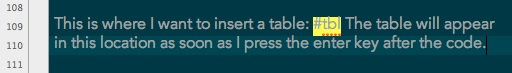
\includegraphics[width=0.5\textwidth]{texnicle-validclip.jpg}
\caption{A valid clip from the library will turn yellow.}
\label{fig:texnicle-validclip}
\end{figure}

Once the shortcut command turns yellow, press \keys{\returnkey} to insert the clip. The |#ben| command (shortcut for an |enumerate| environment) will yield the something like Figure \ref{fig:texnicle-benexpanded} in the editor:
\begin{figure}[htbp]
\centering
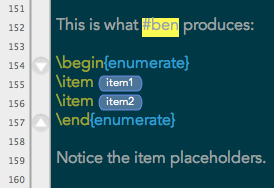
\includegraphics[width=0.3\textwidth]{TeXnicle-Images/texnicle-benexpanded.png}
\caption{An expansion of the code for an \texttt{enumerate} environment.}
\label{fig:texnicle-benexpanded}
\end{figure}

Some clippings, like that in Figure \ref{fig:texnicle-benexpanded} have placeholders that can be replaced by the user. These look like the bubbles ``item1'' and ``item2'' in the figure. In clippings you define yourself, include placeholder text by enclosing the text in \@ symbols. For example, to create a shortcut for text in small caps (the |\smallcaps| command), we will create a new clipping that contains |\textsc{@smallcaps@}|. When the clipping is used (perhaps with a command we define such as |#sc|), the word ``smallcaps'' will appear in a placeholder, as in Figure \ref{fig:texnicle-customclipplaceholder} below.
\begin{figure}[htbp]
\centering
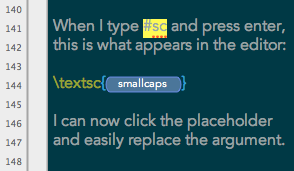
\includegraphics[width=0.3\textwidth]{TeXnicle-Images/texnicle-customclipplaceholder.png}
\caption{After defining a placeholder, this is the output.}
\label{fig:texnicle-customclipplaceholder}
\end{figure}

\section{Bookmarks and Code Folding}
\label{reference.bookmarksfolding}
Two of \texnicle's features are found along the left side of the editor window. Bookmarks are a useful feature of \texnicle that allow you to jump between different parts of your project quickly and easily. Click the line number of the line you want to bookmark, and a blue arrow will appear. Click it again to delete the bookmark. (Alternatively, the keyboard shortcut \keys{\cmdkey + D} will toggle the bookmark on a line.) Under the Information tab of the Navigators pane, the first sub-tab will display all bookmarks in the project grouped by file. Double-click a bookmark to jump to that part of the document. At the top of the editor window, the Jump to Section drop-down menu will show the bookmarks in the current document in relation to labeled sectioning commands in the open document. Both locations are shown in Figure \ref{fig:texnicle-bookmarks}.
\begin{figure}[htbp]
\centering
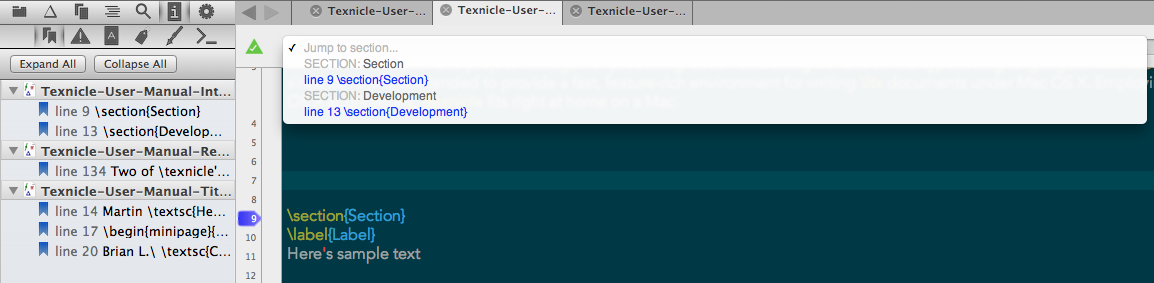
\includegraphics[width=0.75\textwidth]{TeXnicle-Images/texnicle-bookmarks.png}
\caption{Bookmarks in \texnicle shown in the Navigator pane on the left and the Jump to Section menu at the top of the editor window.}
\label{fig:texnicle-bookmarks}
\end{figure}

Note that this feature marks the line number, not the text. For example, if you add five lines before a bookmark on line 20, the bookmark will remain at line 20 while the text that used to be marked will now be located at line 25.

Bookmarks work better if line numbering is turned on; this is controlled under \menu{Preferences\ldots > General}.

Another useful feature of \texnicle is code folding. Environments enclosed by |\begin| and |\end| commands may be collapsed using the arrow buttons between line numbering (if it's turned on) and the editor window, as in Figure \ref{fig:texnicle-codefold}.

\begin{figure}[htbp]
\begin{minipage}{0.55\textwidth}
\begin{flushleft}
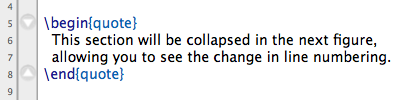
\includegraphics[width=1.0\textwidth]{TeXnicle-Images/texnicle-codefold-open.png}
\end{flushleft}
\end{minipage}
\begin{minipage}{0.45\textwidth}
\begin{flushright}
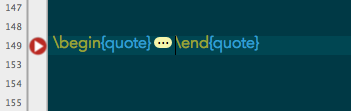
\includegraphics[width=1.0\textwidth]{TeXnicle-Images/texnicle-codefold-closed.png}
\end{flushright}
\end{minipage}
\caption{Code folding: before and after}
\label{fig:texnicle-codefold}
\end{figure}                  
 
When an environment is folded, the fold icon turns red. Notice the jump in line numbering following a fold, as well. The yellow ellipsis icon between |\begin| and |\end| is another indicator that code has been folded. One advantage to having code folding activated is that |\begin| commands without matching |\end| commands are marked with a red X over the code folding arrow.
\begin{figure}[htbp]
\centering
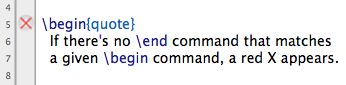
\includegraphics[width=0.5\textwidth]{TeXnicle-Images/texnicle-codefold-nomatch.png}
\caption{An unmatched \textbackslash\texttt{begin} command}
\label{fig:texnicle-codefold-nomatch}
\end{figure}

\section[The Edit Menu]{The \menu{Edit} Menu}
\label{reference.editmenu}
Beyond \menu{Undo}, \menu{Select All}, and \menu{Speech}, the \menu{Edit} menu has a few tricks up its sleeve that should be highlighted, as they are some of \texnicle's most powerful features.

\subsection[Paste as Image]{\menu{Edit > Paste as Image}}
\label{reference.edit.pasteimg}
After copying an image to the pasteboard, you can insert it into \texnicle in a |figure| environment quickly and easily under \menu{Edit > Paste as Image} or with the keyboard shortcut \keys{\ctlkey + \cmdkey + V}. You will be asked to name the image and save it on your hard drive; after that, your image will be inserted in a stock |Figure| environment.

In a project, the image will automatically appear under the last folder in your project tree that was selected. If you want the image to be loaded into a particular folder, click the folder before pasting the image. If you forget to do this, drag the image within the project file list to the desired folder.

\subsection[Paste as Table]{\menu{Edit > Paste as Table}}
\label{reference.edit.pastetab}
Similarly to pasting as an image, \texnicle can convert copied Microsoft Excel\footnote{Martin: Does this apply to Apple Numbers, too? Or other spreadsheet programs? What about Microsoft Word/Apple Pages/other Word Processor table environments?} cells on the pasteboard as a \LaTeX\ table by choosing \menu{Edit > Paste as Table} (keyboard shortcut \keys{\optkey + \cmdkey + V}). You will be asked to select the delimiting character. It is important to remember that while this feature correctly formats the table itself, it does not format the text. Any text formatting, such as correcting Unicode accents, replacing special characters, and editing punctuation, will need to be done by hand.

\noted{Choosing the ``tab'' delimiter will correctly paste the table from Apple Numbers and Microsoft Excel, but other programs and formats may require other delimiters. If your table doesn't paste correctly, try pasting with a different delimiter.}

\subsection[Other Edit Menu Functions]{Other \menu{Edit} Menu Functions}
\label{reference.edit.other}
A few other goodies are included in under \menu{Edit} that should be briefly mentioned. \menu{Edit > Reformat Paragraph} (keyboard shortcut \keys{\ctlkey + Q}) is useful when lines are set to hard wrap rather than soft wrap under \menu{Preferences\ldots > General}. Reformat Paragraph deletes hard-wrap editor line breaks to typeset the entire selection on a single editor line. Lines in the editor still wrap as expected at the set number of characters.

\menu{Edit > Smart Complete} will attempt to complete the word or command you have started typing. It's easily found by pressing \keys{\esckey}.

\menu{Edit > Quick Spell}, also accessible with the keyboard shortcut \keys{\ctlkey + Space}, will pull up a list of words that \texnicle thinks you may be typing based on the characters you have already typed. This is similar to Smart Complete above except that it does not suggest \LaTeX\ commands.

\section[The Editor Menu]{The \menu{Editor} Menu}
\label{reference.editortable}
The \menu{Editor} menu also holds a few less obvious \texnicle features. This section will give a quick overview of their functions.

\menu{Editor > Insert Table} will insert a blank a |tabular| environment (contained within a |table| environment) with a desired number of columns and rows. Placeholders will be inserted in each cell to facilitate editing. An example table with two columns and three rows is shown in Figure \ref{fig:texnicle-inserttable}.

\begin{figure}[htbp]
\centering
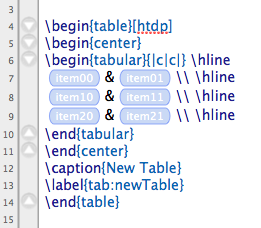
\includegraphics[width=0.3\textwidth]{TeXnicle-Images/texnicle-inserttable.png}
\caption{A table inserted by \texnicle}
\label{fig:texnicle-inserttable}
\end{figure}

\menu{Editor > Insert In-line Math} provides a quick shortcut to inserting math mode (|$ $|) with a placeholder in the middle. More useful is the keyboard shortcut: \keys{\optkey + \shiftkey + \cmdkey + M}.

\menu{Editor > Go To Line\ldots} will allow you to jump within the open document to a particular line or character. The keyboard shortcut is \keys{\cmdkey + L}.

Line indentation, comment level, and jumping between placeholders is all manageable from this menu.

%This menu includes \menu{Increase Indentation} and \menu{Decrease Indentation} commands for changing indentation from the editor margin. Keyboard shortcuts are \keys{\cmdkey + [} to increase and \keys{\cmdkey + ]} to decrease.
%
%Comments are manageable from the \menu{Editor} menu, as well. Click \menu{Toggle Comment} (keyboard shortcut \keys{\cmdkey + /}) to toggle whether a line is commented or not. Use \menu{Increase Comment Level} (shortcut \keys{\optkey + cmdkey + /}) and \menu{Decrease Comment Level} (shortcut \keys{\ctlkey + \cmdkey + /}) to change comment level.
%
%To search for the next placeholder text in the document, click \menu{Editor > Jump to Next Placeholder} or use the keyboard shortcut \keys{\cmdkey + \returnkey}. Similarly, \keys{\shiftkey + \cmdkey + \returnkey} is a shortcut to \menu{Jump to Previous Placeholder}.
